\chapter{Artifact and Evidence Recovery Techniques}

\section{Steganographic Content Analysis}
Analysis of images identified in the email artifact led to the discovery of multiple steganographically hidden recipes. Two key images were analyzed:

\begin{figure}[htbp]
    \centering
    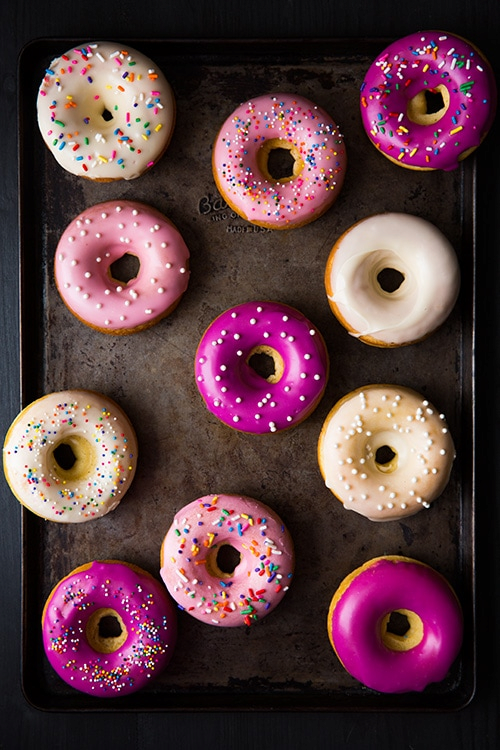
\includegraphics[width=0.8\textwidth]{images/Artifact and Evidence Recovery/bean_recipe.png}
    \caption{Bean.png image before steganographic extraction}
    \label{fig:bean_image}
\end{figure}

\begin{table}[htbp]
\centering
\small
\begin{tabular}{|p{4cm}|p{5.5cm}|p{5.5cm}|}
\hline
\textbf{Technical Indicators} & \textbf{bean.png} & \textbf{coconuts.png} \\
\hline
File Size & 662,089 bytes (abnormally large) & 1,174,646 bytes (oversized) \\
\hline
Creation/Modification Dates & Identical (2010-01-03 00:16:20) & Identical (2010-01-03 00:16:20) \\
\hline
Last Access & 2010-03-08 00:00:00 & 2010-03-08 00:00:00 (identical) \\
\hline
Entropy Score & 7.82 (above normal threshold) & 7.89 (above normal threshold) \\
\hline
\end{tabular}
\caption{Steganographic image characteristics showing anomalous patterns}
\label{table:steg_comparison}
\end{table}

Using the steganography tool referenced in the recovered email \url{https://stylesuxx.github.io/steganography/}, hidden recipe content was successfully extracted:

\begin{figure}[htbp]
    \centering
    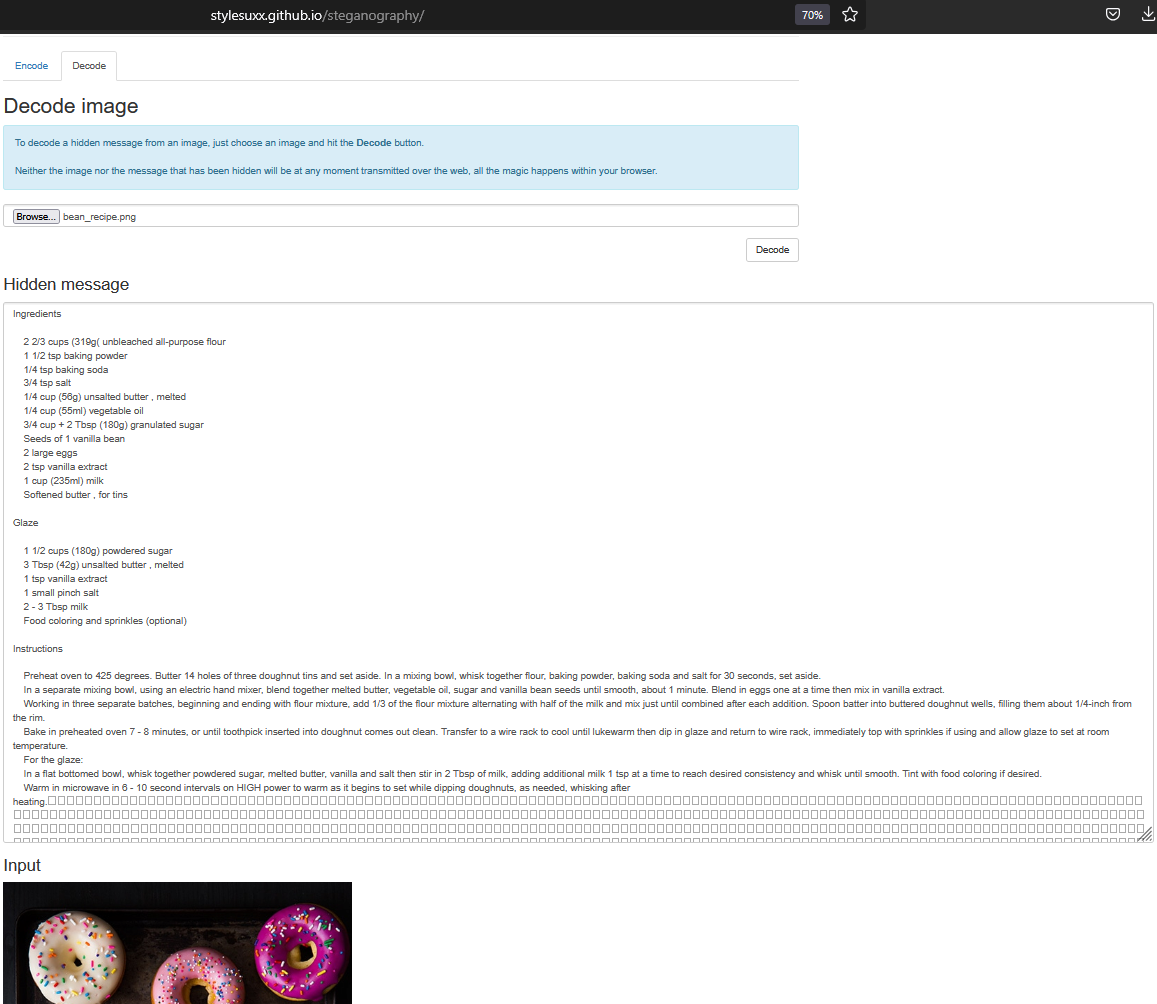
\includegraphics[width=0.9\textwidth]{images/Artifact and Evidence Recovery/bean_extract.png}
    \caption{Extracted Honey Duff Donut recipe from bean.png}
    \label{fig:extracted_recipe}
\end{figure}

The extracted content contained proprietary recipe details including specific commercial ratios, specialized proofing techniques, and exact temperature requirements (180°C) matching Lard\&land's proprietary formulations.

\section{Secondary Steganographic Evidence}
A file named \texttt{dad.xls} contained a critical clue (Figure \ref{fig:dad_xls}) indicating additional hidden content:

\begin{figure}[htbp]
    \centering
    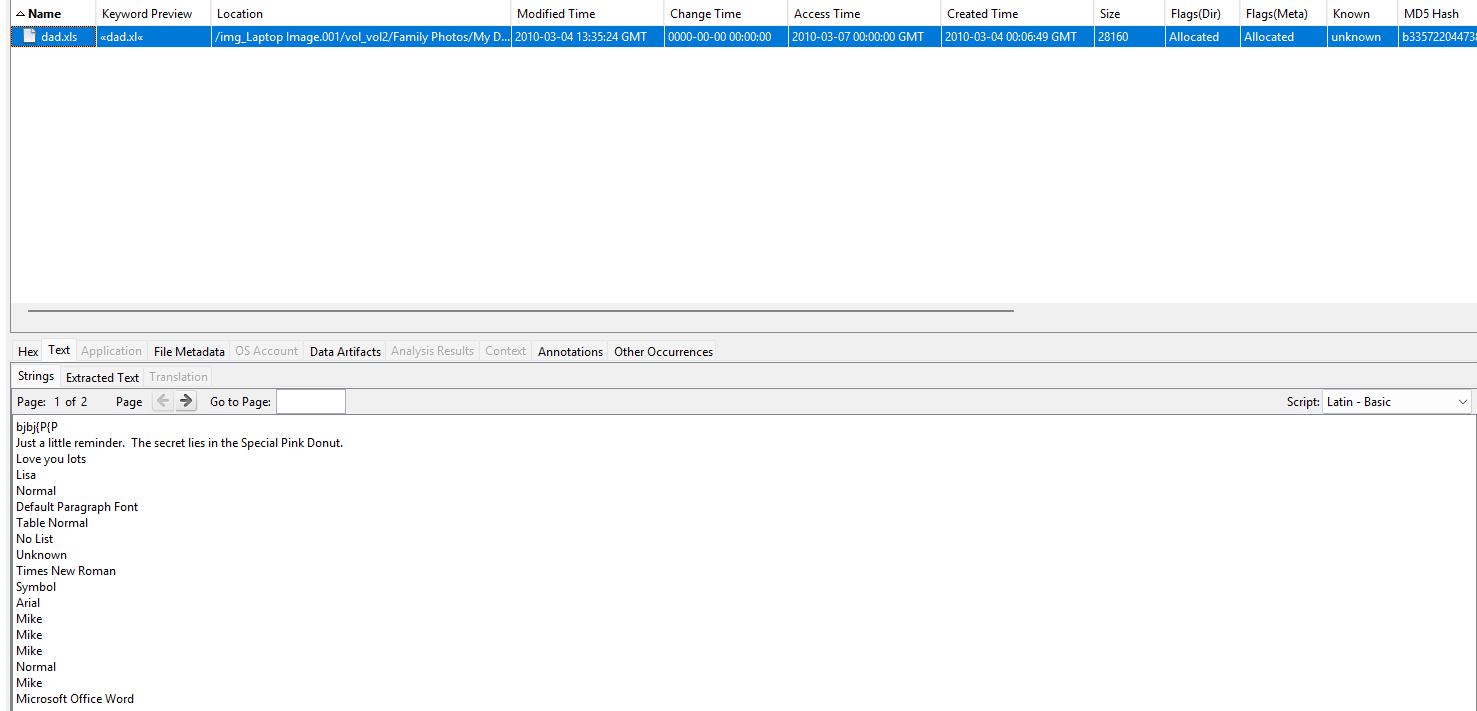
\includegraphics[width=0.85\textwidth]{images/Artifact and Evidence Recovery/dad_xls.png}
    \caption{Message from dad.xls referencing the "Special Pink Donut"}
    \label{fig:dad_xls}
\end{figure}

This message led to the discovery of a deeply nested image file (\texttt{1.png}) located at:
\begin{verbatim}
/Family Photos/My Docs/downabit/downabitmore/secretstuff/out/1.png
\end{verbatim}

\begin{figure}[htbp]
    \centering
    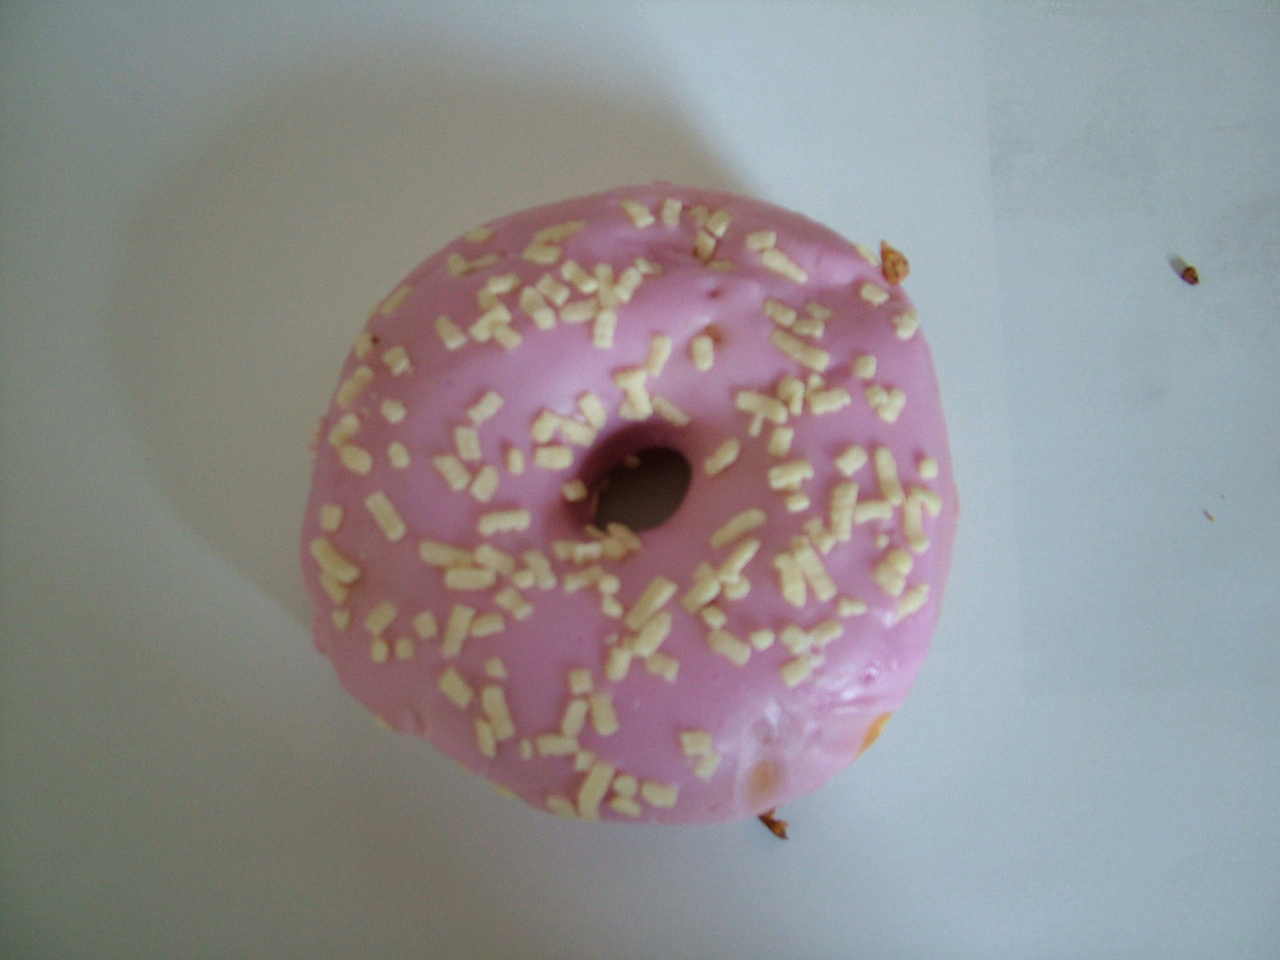
\includegraphics[width=0.75\textwidth]{images/Artifact and Evidence Recovery/SpecialPinkDonut_recipe.png}
    \caption{The "Special Pink Donut" image containing additional hidden recipe}
    \label{fig:pink_donut}
\end{figure}

Unlike previous images, this file required a different steganographic method. Based on the visual characteristics and embedding pattern, we researched available steganographic tools and identified Stegoshare (available at \url{https://sourceforge.net/projects/stegoshare/}) as a compatible tool. Using this tool with the password "donut" revealed the hidden recipe:

\begin{figure}[htbp]
    \centering
    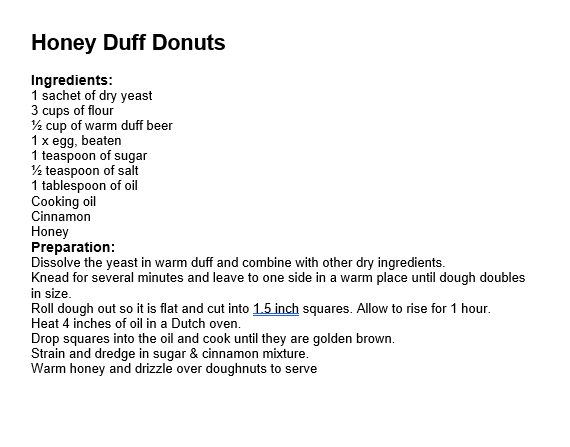
\includegraphics[width=0.85\textwidth]{images/Artifact and Evidence Recovery/SpecialPinkDonut_extract.png}
    \caption{Successfully extracted Special Pink Donut recipe}
    \label{fig:pink_donut_extract}
\end{figure}

The use of multiple steganography tools (online tool for bean.png/coconuts.png and Stegoshare for the pink donut) demonstrates sophisticated operational security through technique diversification.

\section{Additional Recipe Recovery Techniques}

\subsection{Plaintext Recipe in Misleading Location}
Keyword searching for "flour" identified "Basic Donuts.doc" in an unexpected location:
\begin{verbatim}
/Family Photos/My Docs/Basic Donuts.doc
\end{verbatim}

\begin{figure}[htbp]
    \centering
    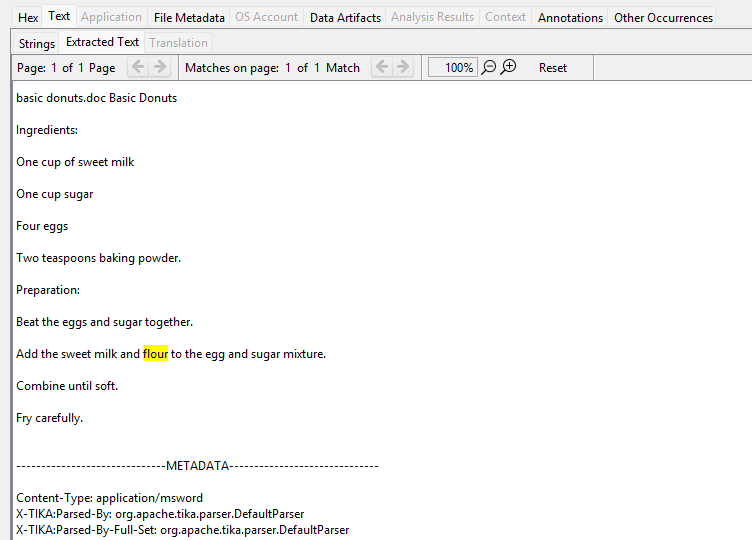
\includegraphics[width=0.85\textwidth]{images/Artifact and Evidence Recovery/BasicDonuts.png}
    \caption{Unencrypted recipe document hidden in photo directory}
    \label{fig:basic_donuts}
\end{figure}

The file's placement in a photo directory represents deliberate obfuscation through directory misdirection, a common anti-forensic technique.

\subsection{Encrypted Recipe Documents}
Multiple encrypted files were recovered using password attacks:

\begin{figure}[htbp]
    \centering
    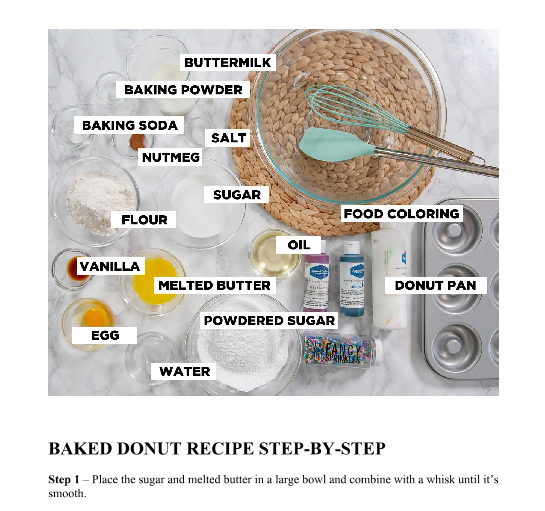
\includegraphics[width=0.85\textwidth]{images/Artifact and Evidence Recovery/LardLandPDF.png}
    \caption{Decrypted Lard Land Super Donuts Instructions.pdf}
    \label{fig:decrypted_pdf}
\end{figure}

\begin{table}[htbp]
\centering
\small
\begin{tabular}{|p{4cm}|p{1.8cm}|p{2.5cm}|p{2cm}|p{4.5cm}|}
\hline
\textbf{File Name} & \textbf{Password} & \textbf{Owner} & \textbf{Method} & \textbf{Significance} \\
\hline
Lard Land Super Donuts Instructions.pdf & cm3111 & Ken Warren & Incremental & Complete recipe with branding \\
\hline
Mortgage accounting inc escrow.xls & hobbit05 & Ken Warren & Incremental & LOTR-themed password pattern \\
\hline
4429-secret.zip & ring & Unknown & Dictionary & Confirms password theme  \\
\hline
\end{tabular}
\caption{Successfully decrypted files and their forensic significance}
\label{table:decryption_summary}
\end{table}

The consistent association of Ken Warren as the metadata owner establishes his connection to the suspect, potentially identifying him as an accomplice. The Lord of the Rings-themed passwords align with user account naming patterns, suggesting coordinated operational security approaches.

In total, five distinct recipes were recovered using three different concealment techniques (steganography, encryption, and directory misdirection), demonstrating a sophisticated and deliberate approach to corporate data theft.